\documentclass{article}

\def\pub{false} % true for publication, false for draft
\newcommand*{\template}{../dding_template}
\input{\template/preamble/preamble_article.tex}

% Definition of \maketitle
\makeatletter         
\def\@maketitle{
    \raggedleft
    
\includegraphics[width = 20mm]{GIST_Logo.jpg}\\[5ex]
    \begin{center}
        {\Huge \bfseries \@title }\\[4ex] 
        {\Large  \@author}\\[4ex] 
        \@date\\[8ex]
    \end{center}
}
\makeatother

\dottedcontents{section}[2em]{\bfseries}{1.5em}{1pc}
\dottedcontents{subsection}[3em]{}{1.7em}{1pc}

% ========================================
\newcommand*{\bdx}{\mv{x}} % bold x
\newcommand*{\bdy}{\mv{u}} % bold u
\newcommand*{\bdz}{\mv{z}} % bold z
\newcommand*{\bdq}{\mv{q}} % bold q

\newcommand*{\bdf}{\mv{f}} % bold f

\newcommand*{\tpfpx}{\pptfrac{\bdf}{\bdx}} % partial f / partial x
\newcommand*{\pfpx}{\ppfrac{\bdf}{\bdx}} % partial f / partial x
% ========================================

% \bibliography{\template/refs.bib}

\title{
    Deep-Neuro Control with Contraction Theory
}

\author{
    Myeongseok Ryu
    \thanks{Myeongseok Ryu and Kyunghwan Choi are with the School of Mechanical and Robotics Engineering, Gwangju Institute of Science and Technology, 61005 Gwangju, Republic of Korea {\tt\small dding\_98@gm.gist.ac.kr, khchoi@gist.ac.kr}}%
    ,
    Sesun You
    \thanks{Sesun You is 
        {\tt\small example@mail.com}}%
    ,
    Kyunghwan Choi
    \footnotemark[1]
}

\date{
    % 20\textsuperscript{th} March 2025
    \today
    \\
    Version 0.0
}

\begin{document}

\maketitle

\begin{abstract}
    This project aims to develop control or estimator with deep neural network and contraction theory.
\end{abstract}

\tableofcontents

% ========================================
%         INTRODUCTION
% ========================================


\section{Introduction}

\subsection{Background}

\subsection{Research Objectives}

The main objectives of this research are as follows:
\begin{itemize}
    \item Mathematical stability analysis of the controller and estimator with deep neural networks using the contraction theory.
    \item Development of the controller and estimator with deep neural networks using the contraction theory.
\end{itemize}

% ========================================
%         NOTATIONS AND PRELIMINARIES
% ========================================

\section{Notations and Preliminaries}

The following notations are used throughout this document:
\begin{itemize}
    \item $:=$ denotes \textit{defined as}.
    \item $(\cdot)^\top$ denotes the transpose of a matrix or a vector.
    \item $\bdx:=[x_i]_{i\in\{1,\cdots,n\}}\in\R^n$ denotes the state vector.
    \item $\mm A:=[a_{ij}]_{i,j\in\{1,\cdots,n\}}\in\R^{n\times n}$ denotes a matrix.
    \item $\lambda_{i}(\mm A),\ i\in\{\max,\min\}$ denotes the maximum and minimum singular value of $\mm A$, respectively.
    \item $\mm I_n$ denotes the identity matrix of size $n$ and $\mm 0_{n\times m}$ denotes the zero matrix of size $n\times m$.
    \item $\mysym$ denotes the symmetric part of a matrix, \ie $\mysym(\mm A):=\tfrac{1}{2}(\mm A+\mm A^\top)$ (see, \cite{Tsukamoto:2021ac}).
\end{itemize}

We introduce the following lemmas.

\begin{lem}[Comparison Lemma]
	Suppose that a continuously differentiable function $f:\R^n\to\R$ satisfies the following inequality:
	\begin{equation}
		\ddtt f(t)\le -a f(t)+ b, \quad \forall t\in\R_{\ge 0}
		,
	\end{equation}
	where $a,b>0$.
	Then, the following inequality holds:
	\begin{equation}
		f(t)\le -af(0)e^{-at} + \tfrac{b}{a}(1-e^{-at}), \quad \forall t\in\R_{\ge 0}
	\end{equation}
	and remains in a compact set $f(t)\in\{\norm{f(t)} \mid \norm{f(0)}\le \tfrac{b}{a}\}$.
	\label{lem:comparison}
\end{lem}

\begin{proof}
	This is a simple special case of the comparison lemma \cite[pp. 102-103]{Khalil:2002aa}.
	See \cite[pp. 659-660]{Khalil:2002aa}.
\end{proof}

% ========================================
%         REVIEW OF CONTRACTION THEORY
% ========================================

\section{Review of Contraction Theory}

For your smooth start, we recommend you to begin with \cite{LOHMILLER:1998aa}.
The overview of contraction theory is presented in a review paper \cite{Tsukamoto:2021aa}.

\subsection{Basic Results of Contraction Theory for Deterministic Systems}

First, we start with the following deterministic systems:
\begin{equation}
    \ddtt{\bdx}
    = 
    \bdf(\bdx,t)
    ,
    \label{eq:sys}
\end{equation}
where $\bdf(\bdx,t)$ is an $n\times1$ sufficiently smooth non-linear vector function and $\bdx\in\R^n$ is the state vector.
The smooth property of $\bdf(\bdx,t)$ is essential to ensure the existence and uniqueness of the solution to \eqref{eq:sys} \cite[see, pp. 88-89]{Khalil:2002aa}.

\begin{figure}[!t]
    \centering
    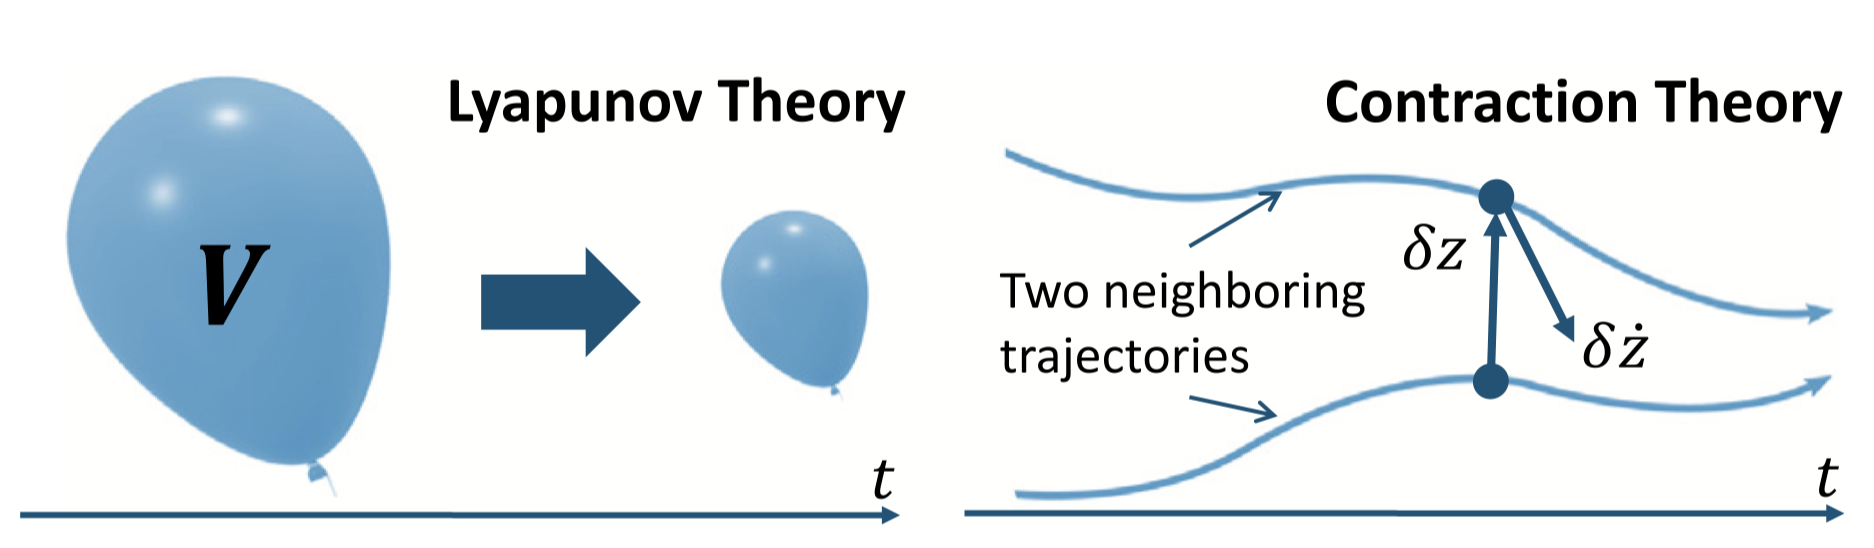
\includegraphics[width=0.5\textwidth]{figs/lyaVSctrac.png}
    \caption{
        Difference between Lyapunov and contraction theory \cite[Fig. 1]{Tsukamoto:2021aa}.
        The Lyapunov theory investigates the convergence to a single point and the contraction theory does regarding a single trajectory.
    }
    \label{fig:lyaVSctrac}
\end{figure}

The biggest difference between the traditional Lyapunov theory and the contraction theory is that the contraction theory investigates the convergence of the state trajectory to a single trajectory (contraction behavior), while the Lyapunov theory focuses on the convergence of the state trajectory to a single point \ie see, Fig.~\ref{fig:lyaVSctrac}.
For this, motivated by the calculus of variations \cite[Chap. 4]{Kirk:2004aa}, \eqref{eq:sys} can be rewritten as differential dynamics using \textit{differential displacement} $\delta\bdx$ as follows:
\begin{equation}
    \ddtt\delta\bdx
    =
    \tpfpx(\bdx,t)
    \delta\bdx
    .
    \label{eq:diff_sys}
\end{equation}
For your information, $\delta\bdx$ is an infinitesimal displacement at \textit{fixed time}.

\subsubsection{Definitions}

Before we present the fundamental theorem of contraction theory, we introduce the following definitions.
One can re-visit this section while reading further.

\begin{definition}[see, Def. 2.2 \cite{Tsukamoto:2021aa}]  
    If any two trajectories $\mv\xi_1(t)$ and $\mv\xi_2(t)$ of \eqref{eq:sys} converge to a single trajectory, then the system \eqref{eq:sys} is said to be \textit{incrementally exponentially stable}, if $\exists C,\alpha>0$, subject to the following holds:
    \begin{equation}      
        \norm{\mv\xi_1(t)-\mv\xi_2(t)}
        \le 
        C
        \norm{\mv\xi_1(0)-\mv\xi_2(0)}
        \exp^{-\alpha t}
        ,\ \forall t\in\R_{\ge 0}
        .
    \end{equation}
    The result of Theorem \ref{thm:ctrac:main} equivalently implies the incremental exponential stability, since we have $\norm{\mv\xi_1(t)-\mv\xi_2(t)}= \norm{\int_{\mv\xi_1(t)}^{\mv\xi_2(t)}\delta\bdx(t)}$.
    \label{def:inc_exp_stable}
\end{definition}

\begin{definition}
    Let $\mm\Theta(\bdx,t)$ be a smooth coordinate transformation of $\delta\bdx$ to $\delta\bdz$, \ie $\delta\bdz = \Theta(\bdx,t)\delta\bdx$.
    Then, a symmetric continuously differentiable matrix $\mm M(\bdx,t):=\mm\Theta(\bdx,t)^\top\mm\Theta(\bdx,t)$ is said to be a \textit{metric} of the system \eqref{eq:sys}.
    \label{def:metric}
\end{definition}

\begin{definition}
    The covariant derivative of $\mv f(\bdx,t)$ in $\delta\bdx$ coordinate is represented as 
    \begin{equation}
        \mm F
        :=
        \left(
            \ddtt\mm\Theta
            +
            \mm\Theta\tpfpx
        \right)
        \mm\Theta^{-1}
        ,
    \end{equation}
    and is called the \textit{generalized Jacobian}.
    This can be easily derived by differentiating $\delta\bdz = \Theta(\bdx,t)\delta\bdx$ with respect to $t$, leading to $\ddtt\bdz=\mm F\bdz$.
    \label{def:gen_jac}
\end{definition}

\subsubsection{Fundamental Theorem of Contraction Theory}

The following theorem presents the fundamental theorem of contraction theory and corresponding necessary and sufficient condition for exponential convergence of the differential system \eqref{eq:diff_sys}.

\begin{theorem}[see, T. 2.1 \cite{Tsukamoto:2021aa}]
    If $
        \exists \mm{M}(\bdx,t)
        =
        \mm\Theta(\bdx,t)^\top
        \mm\Theta(\bdx,t)
        > 0, \forall \bdx,t
    $ where $\mm\Theta(\bdx,t)$ (see, Definition \ref{def:metric}) defines a smooth coordinate transformation of $\delta\bdx$ to $\delta\bdz$, \ie $\delta\bdz = \Theta(\bdx,t)\delta\bdx$, subject to the following equivalent conditions holds for $\exists\alpha\in\R_{>0},\ \forall \bdx,t$:
    \begin{subequations}
        \begin{align}
            \lambda_{\max} (
                \mm F(\bdx,t)
            )
            =
            \lambda_{\max} 
            \left(
                \left(    
                \ddtt \mm\Theta
                +
                \mm\Theta\tpfpx
                \right)
                \mm\Theta^{-1}
            \right)
            \le&
            -\alpha
            ,
        \label{eq:ctrac:metric:F}
            \\
            \ddtt \mm M
            +
            \mysym(\mm M\tpfpx)
            \le&
            -2\alpha\mm M
            ,
        \label{eq:ctrac:metric:M}
        \end{align}
        \label{eq:ctrac:metric}
    \end{subequations}
    where the arguments of $\mm M(\bdx,t)$ and $\mm F(\bdx,t)$ are omitted for simplicity, then, the system \eqref{eq:sys} is said to be contracting with an exponential rate $\alpha$, \ie all trajectories of \eqref{eq:sys} converge to a single trajectory.
    The converse is also true.
    \label{thm:ctrac:main}
\end{theorem}

\begin{proof}
    Taking time derivative of a differential Lyapunov function of $\delta\bdx$, $V=\delta\bdz^\top\bdz=\delta\bdx^\top\mm M\delta\bdx$, using the differential dynamics \eqref{eq:diff_sys}, we have
    \begin{equation}
        \begin{aligned}
            \ddtt V (\bdx, \delta\bdx, t)
            =&
            \delta\bdx^\top
            \left(
                \ddtt\mm M
                +
                \mysym(\mm M\tpfpx)
            \right)
            \delta\bdx
            =
            2
            \delta\bdz^\top
            \mm F
            \delta \bdz
            \\
            \le&
            -2\alpha
            \delta\bdx^\top
            \mm M
            \delta\bdx
            =
            -
            2\alpha
            \delta\bdz^\top
            \delta\bdz
            =
            -2\alpha V
            .
        \end{aligned}
    \end{equation}
    According to the comparison lemma (Lemma \ref{lem:comparison}), we have $V(t)\le V(0)e^{-2\alpha t}$, which then yields $\norm{\delta\bdz(t)}^2\le\norm{\delta\bdz(0)}^2e^{-2\alpha t}$ and $\norm{\delta\bdz(t)}\le\norm{\delta\bdz(0)}e^{-\alpha t}$.
    This implies that any infinitesimal displacement $\delta\bdz$ and $\delta\bdx$ converges to zero exponentially with rate $\alpha$.
    Note that the initial conditions are exponentially "forgotten" as time goes on.
    The proof of the converse can be found in \cite[Sec. 3.5]{LOHMILLER:1998aa}.
\end{proof}

It is notable that the unboundedness of the metric $\mm M(\bdx, t)$ does not create any problem in a technical sense.
This is because, the dynamics of $\mm M(\bdx, t)$ is linear with infinite escape time.
Therefore, it can be handled by renormalizing the metric $\mm M(\bdx, t)$.

\hfill

Theorem \ref{thm:ctrac:main} can also be proven by using the transformed squared length integrated over two arbitrary solutions of \eqref{eq:sys}.
The following theorem presents the alternative proof of Theorem \ref{thm:ctrac:main}.

\begin{theorem}[see, p. 688 \cite{LOHMILLER:1998aa}, T. 2.3 \cite{Tsukamoto:2021aa}]
    Let $\mv{\xi}_1(t)$ and $\mv{\xi}_2(t)$ be two solutions of \eqref{eq:sys}, and define the transformed squared length with $\mm M(\bdx,t)$ of Theorem \ref{thm:ctrac:main} as follows:
    \begin{equation}
        V_{sl}(\bdx,\delta\bdx,t)
        =
        \textstyle\int_{\mv{\xi}_1(t)}^{\mv{\xi}_2(t)}
        \norm{\delta\bdz}^2
        =
        \textstyle\int_0^1
        \pptfrac{\bdx}{\mu}^\top
        \mm M(\bdx,t)
        \pptfrac{\bdx}{\mu}
        \der\mu
        ,
        \label{eq:Vsl}
    \end{equation}
    where $\bdx$ is a smooth path parameterized as $\bdx(\mu=0,t)=\mv\xi_1(t)$ and $\bdx(\mu=1,t)=\mv\xi_2(t)$ by $\mu\in\{0,1\}$.
    Also, define the path integral with the transformation $\mm\Theta(\bdx,t)$ for $\mm M(\bdx,t)=\mm\Theta(\bdx,t)^\top\mm\Theta(\bdx,t)$ as follows:
    \begin{equation}
        V_{l}(\bdx,\delta\bdx,t)
        =
        \textstyle\int_{\mv{\xi}_1(t)}^{\mv{\xi}_2(t)}
        \norm{\delta\bdz}
        =
        \textstyle\int_{\mv{\xi}_1(t)}^{\mv{\xi}_2(t)}
        \norm{\mm\Theta(\bdx,t)\delta\bdx}
        .
        \label{eq:Vl}
    \end{equation}
    Then, \eqref{eq:Vsl} and \eqref{eq:Vl} satisfy the following inequality:
    \begin{equation}
        \norm{\mv\xi_1(t)-\mv\xi_2(t)}
        =
        \norm{
            \textstyle\int_{\mv{\xi}_1(t)}^{\mv{\xi}_2(t)}
            \delta\bdx
        }
        \le
        \tfrac{V_{l}}{\sqrt{\underbar{m}}}
        \le
        \sqrt{\tfrac{V_{sl}}{\underbar{m}}}
        ,
        \label{eq:xi_x_Vl_Vsl}
    \end{equation}
    where $\mm M(\bdx,t) \ge \underbar{m}\mm I_n,\ \forall \bdx, t$ for $\exists\underbar{m}\in\R_{>0}$ and Theorem \ref{thm:ctrac:main} can also be proven by using \eqref{eq:Vsl} and \eqref{eq:Vl} as a Lyapunov-like function, resulting in incremental exponential stability of the system \eqref{eq:sys} (see, Definition \ref{def:inc_exp_stable}).
    Note that the shortest path integral $V_l$ of \eqref{eq:Vl} with a parameterized state $\bdx$ (\ie $\inf{V_l}=\sqrt{\inf{V_{sl}}}$) defines the Riemannian distance and the path integral of a minimizing geodesic.
    \label{thm:ctrac:path_int}
\end{theorem}

\begin{proof}
    Note that $\mv{\xi}_i(t),\ \forall i\in\{1,2\}$ are parameterized $\bdx$.
    Therefore, left-side equailty of \eqref{eq:xi_x_Vl_Vsl} holds.
    The right-side inequality of \eqref{eq:xi_x_Vl_Vsl} can be proven by using the Cauchy-Schwarz inequality.

    On the other hands, by taking time derivative of $V_{sl}$ and $V_l$, we have $\ddtt V_{sl} \le -2\alpha V_{sl}$ and $\ddtt V_l \le -\alpha V_l$.
    As $\mm{M}(\bdx,t)$ is from Theorem \ref{thm:ctrac:main}, the incremental exponential stability of the system \eqref{eq:sys} is guaranteed using the comparison lemma of Lemma \ref{lem:comparison} as follows: 
    \begin{equation}
        \norm{\mv\xi_1(t)-\mv\xi_2(t)}
        \le
        \tfrac{V_{l}(0)}{\sqrt{\underbar{m}}} \exp(-\alpha t)
        .
    \end{equation}
\end{proof}

In conclusion, Theorem \ref{thm:ctrac:main} defines necessary and sufficient conditions of incremental exponential stability of the system \eqref{eq:sys}, and Theorem \ref{thm:ctrac:path_int} provides an alternative proof of Theorem \ref{thm:ctrac:main} using the path integral of a minimizing geodesic.

\hfill

We provide two simple examples of the contraction system.

\begin{example}[see, Ex. 2.2 \cite{Tsukamoto:2021aa}]
    Consider the following system:
    \begin{equation}
        \dot x = -x +\exp(t)
        .
    \end{equation}
    The differential dynamics of the system can be rewritten as \eqref{eq:diff_sys} with $\delta\bdx=\delta x$ as follows:
    \begin{equation}
        \ddtt\delta x
        =
        -\delta x
        .
    \end{equation}
    Using constraint \eqref{eq:ctrac:metric:M}, one can select the metric $\mm M=I$.
    Then, one can conclude that the system \eqref{eq:sys} is contracting with an exponential rate $\alpha=1$.
    However, the system \eqref{eq:sys} is not stable, since the solution of the system \eqref{eq:sys} is $x(t) = \tfrac{\exp(t)}{2}+(x(0)-\tfrac{1}{2})\exp(-t)$.
    \label{ex:div}
\end{example}

\begin{example}[see, Ex. 1 \cite{Jouffroy:2004aa}]
    Consider the following system:
    \begin{equation}
        \ddtt
        \begin{bmatrix}
            x_1\\
            x_2
        \end{bmatrix}
        =
        \begin{bmatrix}
            -1 & x_1\\
            -x_1 & -1
        \end{bmatrix}
        \begin{bmatrix}
            x_1\\
            x_2
        \end{bmatrix}
        .
    \end{equation}
    Using Lyapunov function $V=\tfrac{1}{2}(x_1^2+x_2^2)$, UGES (Uniformly Globally Exponentially Stable) can be easily proven.
    The differential dynamics of the system can be rewritten as \eqref{eq:diff_sys} with $\delta\bdx=\begin{bmatrix}\delta x_1 & \delta x_2\end{bmatrix}^\top$ as follows:
    \begin{equation}
        \ddtt
        \begin{bmatrix}
            \delta x_1\\
            \delta x_2
        \end{bmatrix}
        =
        \begin{bmatrix}
            -1+x_2 & x_1\\
            -2x_2 & -1
        \end{bmatrix}
        \begin{bmatrix}
            \delta x_1\\
            \delta x_2
        \end{bmatrix}
        .
    \end{equation}
    Even though the system is UGES, it is difficult to prove the contraction of the system, since the skew-symmetric structure of the system matrix is destroyed ub derivation process.

    Alternatively, one can use Lyapunov function $V=\tfrac{1}{2}((x_1-x_1')^2+(x_2-x_2')^2))$ where $x_1'$ and $x_2'$ denotes another solution.
    Hence, the contraction should be compared to an \textit{incremental} form of stability.
\end{example}

\hfill

However, as discussed in Example \ref{ex:div}, aforementioned theorems are limited to the convergence of the state trajectory to a single trajectory.
In the next section, we introduce the partial contraction theory to investigate the convergence of the state trajectory to a desired trajectory.

\subsubsection{Partial Contraction Theory}

The following theorem presents the partial contraction theory to ensure the convergence of the state trajectory to a desired trajectory.

\begin{theorem}[see, T. 1 \cite{Wang:2004aa}, T. 3 \cite{Jouffroy:2004aa}, T. 2.2 \cite{Tsukamoto:2021aa}]
    Consider a nonlinear system of the form 
    \begin{equation}
        \ddtt \bdx = \bdf(\bdx,\bdx,t)
        ,
    \end{equation}
    and assume that the virtual system
    \begin{equation}
        \ddtt\bdq = \bdf(\bdq,\bdx,t)
        ,
    \end{equation}
    is contracting with respect to $\bdq$.
    If a particular solution of the virtual $\bdq$-system verifies a smooth specific property, then all solutions of the original $\bdx$-system verifies this property exponentially.
    The original system is said to be partially contracting.
    \label{thm:ctrac:partial}
\end{theorem}

\begin{proof}
    The virtual, observer-like $\bdq$-system has two particular solutions, namely $\bdq(t) = \bdx(t),\ \forall t\in\R_{\ge0}$ and the solution with the specific property.
    Since all trajectories of the $\bdq$-system converge exponentially to a single trajectory, this implies that $\bdx(t)$ verifies the specific property exponentially.
\end{proof}

I am sure that you cannot easily undertand the word \textbf{specific property} in Theorem \ref{thm:ctrac:partial}.
I hope the following example helps you to understand the partial contraction theory.

\begin{example}[see, Ex. 4 \cite{Jouffroy:2004aa}]
    Consider the system 
    \begin{equation}
        \ddtt \bdx = -\mm D(\bdx) + \bdu,
    \end{equation}
    and reference system 
    \begin{equation}
        \ddtt \bdx_d = -\mm D(\bdx_d).
    \end{equation}
    Using control input $\bdu = -\mm K(\bdx)(\bdx-\bdx_d)+(\mm D(\bdx)-\mm D(\bdx_d))\bdx_d$, the virtual system can be rewritten as
    \begin{equation}
        \ddtt\bdq=-\mm D(\bdx)+\mm K(\bdx)(\bdq-\bdx_d)-\mm D(\bdx_d)\bdx_d
        .
    \end{equation}
    The particular solutions of the virtual system are $\bdq(t)=\bdx(t)$ and \textbf{specific property} $\bdq(t)=\bdx_d(t)$.
    Now, investigate the contraction of the virtual system with the differential dynamics of $\delta\bdq$ as follows: $\ddtt\delta\bdq=-(\mm D(\bdx)+\mm K(\bdx))\delta\bdq$.
    With contraction metric $\mm M=I$ (\ie $\mm D(\bdx)+\mm K(\bdx)>0$), one can conclude that the virtual system is contracting with an exponential rate $\alpha=1$.

    This implies that all solutions including two solutions (\ie $\bdq(t)=\bdx(t)$ and $\bdq(t)=\bdx_d(t)$), of the virtual system will converge to a single trajectory exponentially, leading to $\bdq(t)=\bdx(t)=\bdx_d(t)$.
    
    It is notable that the selection of the virtual system is crucial to simply obtain contraction metric $\mm M(\bdx,t)$.
    If we select the virtual system as $\ddtt \bdq = -(\mm D(\bdq)+\mm K(\bdq))(\bdq-\bdx_d)-\mm D(\bdx_d)\bdx_d$, then the contraction metric $\mm M$ is not easily obtained, since $\pptfrac{\mm K}{\bdq}$ and $\pptfrac{\mm D}{\bdq}$ are not zero matrices.
\end{example}
    
\subsubsection{Derterministic Perturbation}

Let us define deterministic prerturbated system by adding a bounded perturbation $\bdd(\bdx,t)$ to the system \eqref{eq:sys} as follows:
\begin{equation}
    \ddtt\bdx
    =
    \bdf(\bdx,t)
    +
    \bdd(\bdx,t)
    ,
    \label{eq:sys:pert}
\end{equation}
and two solutions of \eqref{eq:sys} $\mv\xi_1(t)$ and \eqref{eq:sys:pert} $\mv\xi_2(t)$.
By parameterzing virtual state $\bdq(\mu,t)$ with $\mu\in[0,1]$ such that $\bdq(\mu=0,t)=\xi_0$ and $\bdq(\mu=1,t)=\xi_1$, we have virtual system as follows:
\begin{equation}
    \ddtt\bdq = \bdf(\bdq(\mu,t),t)+d_\mu(\mu,\xi_1,t)
    ,
    \label{eq:sys:pert:virtual}
\end{equation}
where $d_\mu(\mu,\xi_1,t)=\mu d(\xi_1,t)$, whose particular solutions are $\bdq(\mu=0,t)=\xi_0$ and $\bdq(\mu=1,t)=\xi_1$.

The following theorem states the robustness of contracting system to the deterministic perturbation by extending Theorem \ref{thm:ctrac:path_int}.

\begin{theorem}[see, Eq. 15 \cite{LOHMILLER:1998aa}, Lemma 1 \cite{Dani:2015aa}, T. 2.4 \cite{Tsukamoto:2021aa}]
    If the system \eqref{eq:sys} satisfies \eqref{eq:ctrac:metric} of Theorem \ref{thm:ctrac:main}, then the path integral of the virtual system \eqref{eq:sys:pert:virtual} (\ie $V_l(\bdq,\delta\bdq,t)=\int_{\mv\xi_1}^{\mv\xi_2}\norm{\mm\Theta(\bdq,t)\delta\bdq}$), where $\mv{\xi}_1(t)$ and $\mv{\xi}_2(t)$ are solutions of \eqref{eq:sys} and \eqref{eq:sys:pert}, respectively, converges to a bounded error ball as long as $\mm\Theta\bdd\in \mathcal{L}_\infty$.
    Specifically, if $\exists \underbar m, \bar m\in\R_{>0}$ such that $\underbar m\mm I_n\le\mm M(\bdx,t)\le\bar m\mm I_n$, and $\bar d = \sup_{\bdx,t} \norm{\bdd(\bdx,t)}$, then the following inequality holds:
    \begin{equation}
        \norm{\mv\xi_1(t)-\mv\xi_2(t)}
        \le
        \tfrac{V_{l}(0)}{\sqrt{\underbar{m}}}
        \exp(-\alpha t)
        +
        \tfrac{\bar d}{\alpha}
        \sqrt{\tfrac{\bar m}{\underbar m}}
        (1-\exp(-\alpha t))
        ,
    \end{equation}
    where $V_l(t)=V_l(\bdq,\delta\bdq,t)$.
    \label{thm:ctrac:pert}
\end{theorem}

\begin{proof}
    Invoking $\ddtt(\pptfrac{\bdq}{\mu})=\pptfrac{\bdf}{\bdq}\pptfrac{\bdq}{\mu}+\bdd$ and $\mm M=\mm\Theta^\top\mm\Theta$, we have time derivative integrand of $V_l$ as follows:
    \begin{equation}
        \begin{aligned}
            \ddtt \norm{\mm\Theta\pptfrac{\bdq}{\mu}}
            =&
            \tfrac{1}{2}
            \left(
                \pptfrac{\bdq}{\mu}^\top
                \mm M
                \pptfrac{\bdq}{\mu}
            \right)^{-\tfrac{1}{2}}
            \left[
                \pptfrac{\bdq}{\mu}^\top
                \ddtt \mm M
                \pptfrac{\bdq}{\mu}
                +
                \pptfrac{\bdq}{\mu}^\top
                \mysym(\mm\Theta\tpfpx)
                \pptfrac{\bdq}{\mu}
                +
                \pptfrac{\bdq}{\mu}^\top
                2
                \mm M \bdd            
            \right]
            \\
            \le&
            \tfrac{1}{2}
            \left(
                \pptfrac{\bdq}{\mu}^\top
                \mm M
                \pptfrac{\bdq}{\mu}
            \right)^{-\tfrac{1}{2}}
            \left[
            -2\alpha 
            \pptfrac{\bdq}{\mu}^\top
            \mm M
            \pptfrac{\bdq}{\mu}
            +
            \pptfrac{\bdq}{\mu}^\top
            2
            \mm M \bdd            
            \right]
            \\
            \le &
            -\alpha
            \norm{\mm\Theta\pptfrac{\bdq}{\mu}}
            +
            \norm{\mm\Theta\pptfrac{\bdq}{\mu}}^{-1}
            \norm{\mm\Theta\pptfrac{\bdq}{\mu}}
            \norm{\mm\Theta \bdd}
            \\
            \le &
            -\alpha
            \norm{\mm\Theta\pptfrac{\bdq}{\mu}}
            +
            \norm{\mm\Theta \bdd}
            .
        \end{aligned}
    \end{equation}
    By integrating the above inequality with respect to $\mu$ from $0$ to $1$, we have $\ddtt V_l(t)=-\alpha V_l(t)+\sup_{\bdq,\mv\xi_1,t}\norm{\mm\Theta\bdd}$.
    Hence, by applying the comparison lemma (Lemma \ref{lem:comparison}), we have the following result as follows:
    \begin{equation}
        V_l(t)
        \le
        V_l(0)\exp(-\alpha t)
        +
        \tfrac{\sup_{\bdq,\mv\xi_1,t}\norm{\mm\Theta\bdd}}{\alpha}
        (1-\exp(-\alpha t))
        .
    \end{equation}
    By using the inequality \eqref{eq:xi_x_Vl_Vsl}, we have the desired result as follows:
    \begin{equation}
        \norm{\mv\xi_1(t)-\mv\xi_2(t)}
        \le
        \tfrac{V_{l}(0) \exp(-\alpha t)}{\sqrt{\underbar{m}}}
        +
        \tfrac{\bar d}{\alpha}
        \sqrt{\tfrac{\bar m}{\underbar m}}
        (1-\exp(-\alpha t))
        ,
    \end{equation}
    where $\underbar m=\inf_t\lambda_{\min}(\mm M)$ and $\bar m=\sup_t\lambda_{\max}(\mm M)$.
    It is notable that Theorem \ref{thm:ctrac:path_int} is a special case of Theorem \ref{thm:ctrac:pert} with $\bdd=\mv 0$.
\end{proof}

Since most of systems are subject to the perturbation, Theorem \ref{thm:ctrac:pert} will be utilized in the most of further cases.

\subsection{Basic Results of Contraction Theory for Stochastic Systems}

\color{red}
WILL BE UPDATED LATER.
\color{black}

% ========================================
%         Conclusion
% ========================================
\section{Conclusion}


% ========================================
%         Appendix
% ========================================
\begin{appendices}
% \section{Notable Lemmas}
\end{appendices}

\bibliographystyle{ieeetr}
\bibliography{\template/refs}

% \printbibliography

\end{document}